\documentclass[tikz]{standalone}
\usepackage[T1]{fontenc}
\usepackage{mathpazo} % Palatino font
\usepackage{pgfplots}
\pgfplotsset{compat=1.18}

\begin{document}
	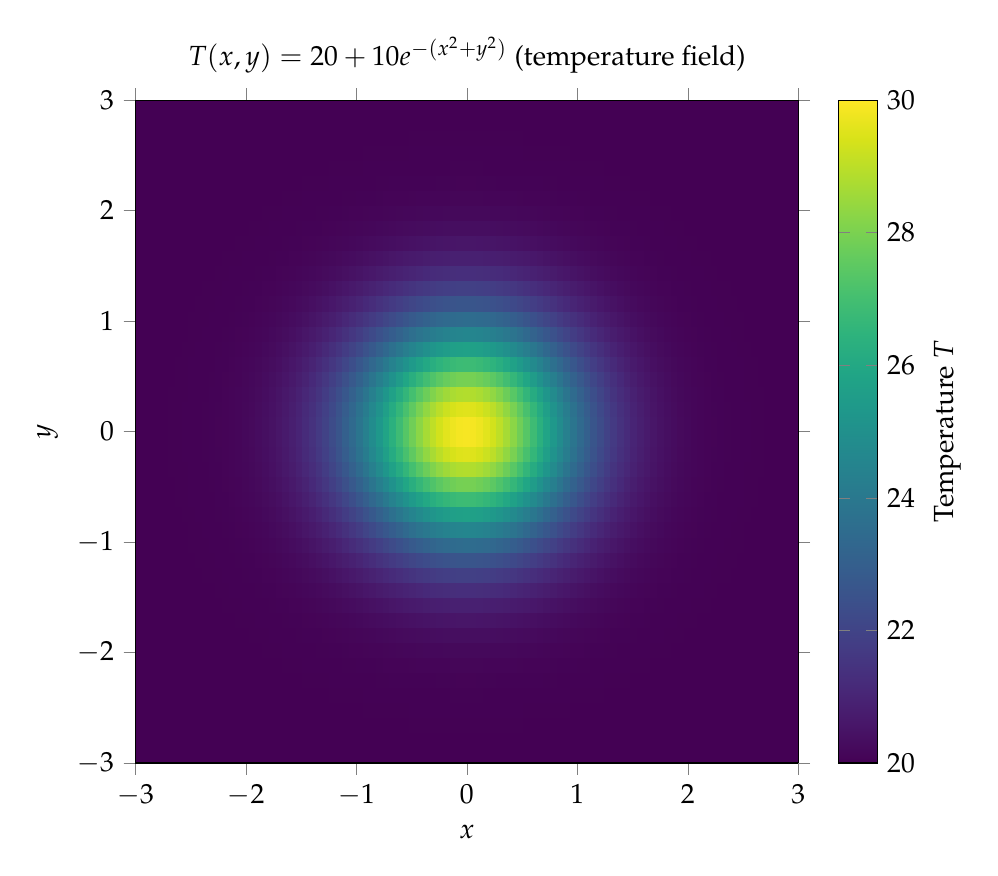
\begin{tikzpicture}
		\begin{axis}[
			width=12cm,
			height=10cm,
			view={0}{90},
			axis equal image,
			xmin=-3, xmax=3,
			ymin=-3, ymax=3,
			xlabel={$x$},
			ylabel={$y$},
			title={$T(x,y)=20+10e^{-(x^2+y^2)}$ (temperature field)},
			colorbar,
			colormap/viridis,
			point meta min=20,
			point meta max=30,
			colorbar style={ylabel={Temperature $T$}, ytick={20,22,24,26,28,30}},
			ticks=both,
			tick align=outside,
			]
			
			% Heatmap (2D scalar field rendered as a top-down surface)
			\addplot3[
			surf,
			shader=flat,
			draw=none,
			domain=-3:3,
			y domain=-3:3,
			samples=100,
			samples y=45,
			]
			{20 + 10*exp(-(x^2+y^2))};
			
			% Isotherms are circles because T depends only on r^2 = x^2+y^2.
			% Levels 21..29 -> radii r = sqrt(-ln((L-20)/10)).
			% Precomputed radii (approx): 21:1.5174 22:1.2686 23:1.0973 24:0.9572
			% 25:0.8326 26:0.7147 27:0.5972 28:0.4724 29:0.3246
%			\foreach \r/\lab in {1.5174/21,1.2686/22,1.0973/23,0.9572/24,0.8326/25,0.7147/26,0.5972/27,0.4724/28,0.3246/29}{
%				\addplot[black, thick, samples=240, domain=0:360]
%				({\r*cos(x)},{\r*sin(x)});
%				% optional label (comment out if you want cleaner look)
%%				\node[black, fill=white, inner sep=1pt] at (axis cs:{\r},0) {\scriptsize $\lab^\circ$};
%			}
			
%			% Mark peak
%			\addplot[only marks, mark=*, mark size=2pt] coordinates {(0,0)};
%			\node[anchor=south east] at (axis cs:0,0) {$T(0,0)=30$};
			
		\end{axis}
	\end{tikzpicture}
\end{document}
